\documentclass{beamer}
\usepackage{default}
\usepackage{amsmath}
\usepackage{graphicx}
\usepackage{adjustbox}  % Allows for fitting tables into slide
%\usepackage{hyperref}
\usepackage{threeparttable}
\usepackage{caption}
%\usepackage{subcaption}
\usepackage{natbib}
\usepackage{adjustbox}
\usepackage{subcaption}
\usepackage{hyperref}
\hypersetup{
	colorlinks = true,
	linkcolor=.,
	citecolor= {cyan}
}



%\usetheme{AnnArbor}
%\usetheme{Antibes}
%\usetheme{Bergen}
%\usetheme{Berkeley}
%\usetheme{Berlin}
%\usetheme{Boadilla}
%\usetheme{boxes}
\usetheme{CambridgeUS}
%\usetheme{Copenhagen}
%\usetheme{Darmstadt}
%\usetheme{default}
%\usetheme{Frankfurt}
%\usetheme{Goettingen}
%\usetheme{Hannover}
%\usetheme{Ilmenau}
%\usetheme{JuanLesPins}
%\usetheme{Luebeck}
%\usetheme{Madrid}
%\usetheme{Malmoe}
%\usetheme{Marburg}
%\usetheme{Montpellier}
%\usetheme{PaloAlto}
%\usetheme{Pittsburgh}
%\usetheme{Rochester}
%\usetheme{Singapore}
%\usetheme{Szeged}
%\usetheme{Warsaw}

% colortheme to choose one 

%\usecolortheme{beaver}
%\usecolortheme{crane}
%\usecolortheme{default}
\usecolortheme{dolphin}
%\usecolortheme{seagull}
%\usecolortheme{seahorse}
%\usecolortheme{whale}


% fond theme to choose one 
%\usefonttheme{structuresmallcapsserif}
%\usefonttheme{structureitalicserif}
%\usefonttheme{structurebold}
\usefonttheme{serif}
%\usefonttheme{professionalfonts}
%\usefonttheme{default}

\title{Perceived Income Risks and Subjective Attribution}


% A subtitle is optional and this may be deleted

\author{Tao Wang \\ Johns Hopkins University}
% - Give the names in the same order as the appear in the paper.
% - Use the \inst{?} command only if the authors have different
%   affiliation.

\date{\today}
% - Either use conference name or its abbreviation.
% - Not really informative to the audience, more for people (including
%   yourself) who are reading the slides online

% This is only inserted into the PDF information catalog. Can be left
% out. 

% If you have a file called "university-logo-filename.xxx", where xxx
% is a graphic format that can be processed by latex or pdflatex,
% resp., then you can add a logo as follows:

% \pgfdeclareimage[height=0.5cm]{university-logo}{university-logo-filename}
% \logo{\pgfuseimage{university-logo}}

% Delete this, if you do not want the table of contents to pop up at
% the beginning of each subsection:
\AtBeginSubsection[]
{
	\begin{frame}<beamer>{Outline}
	\tableofcontents[currentsection]
\end{frame}
}

\begin{document}
	

\begin{frame}
	\titlepage
\end{frame}
\begin{frame}{Outline}
	\tableofcontents
	% You might wish to add the option [pausesections]
\end{frame}


\section{Motivation}

%\begin{frame}{Motivation}
%	\begin{itemize}
%		\item Risks matter for individual decisions
%		\begin{itemize}
%			\item precautionary saving
%			\item portfolio choice and stock market participation
%		\end{itemize} 
		%%Not just expectation of income but also \textcolor{blue}{high moments} such as income risks matter for consumption/portfolio decisions, i.e. precautionary motives, stock market investment, etc. 
%		\item Risks matter for macroeconomic outcomes
%		\begin{itemize}
%			\item Since idiosyncratic risks are not perfectly insured 
%			\item Different wealth $\rightarrow$ different MPCs $\rightarrow$ distributional channel of macroeconomic policies 
%		\end{itemize}  %%\textcolor{blue}{Uninsurance} of idiosyncratic risks make it matter in macroeconomics, i,e. the important assumption by the HANK literature  
%		\item \textcolor{red}{Risks estimated from cross-sectional microdata $\approx$  ``the truth''  $\approx$ perceptions?} %%It is unclear if perceptions consistent with econometricians' estimates of income risks from cross-sectional inequality and the those used in structural models   What enter in people's calculation are \textcolor{blue}{perceived} risks 
%		%%People make  their decisions based on there \textit{their} perceptions
%	\end{itemize}
%\end{frame}


\begin{frame}{This paper's agenda}
	
	\begin{enumerate}
		\item \textbf{Theory}: a \textcolor{blue}{subjective} heterogeneous-agent model 
		\begin{itemize}
			\item  \textcolor{blue}{imperfect understanding} of income risks
			\begin{itemize}
				\item the \textcolor{blue}{size:} experienced volatility $\rightarrow$  perceived risks
				\item the \textcolor{blue}{nature:} i.e.  aggregate v.s. idiosyncratic  $\rightarrow$ different perceptions
			\end{itemize}
			\item life-cycle agents with uninsured idioyncratic (and aggregate) risks
		\end{itemize} 
		\item \textbf{Empirics:} subjective risk perceptions from density surveys
		\begin{itemize}
			\item \textcolor{blue}{Cross-sectional difference} across \textcolor{red}{age, generation and income} 
			\item \textcolor{blue}{Correlation structure} with current labor market outcomes: \textcolor{red}{counter-cylical} 
			%\item \textcolor{blue}{Time series property}: i.e. how persistent?
			%\item \textcolor{blue}{Decision implications}, i.e. higher perceived risk $\rightarrow$ higher precautionary saving 
			%\item differ systematically by \textcolor{blue}{income, age, generation,  and education}
			%\item affect  \textcolor{blue}{planned spendings} 
			%\item non-normality, i.e half of population have
			%\textcolor{blue}{non-zero skewness}
			%\item \textcolor{blue}{negatively correlate with stock market returns}
			% \item how persistent? (work in progress)
		\end{itemize}
		
	\end{enumerate}
\end{frame}
\begin{frame}{Literature}
	\begin{itemize}
		\item experience-based learning: \cite{malmendier2015learning} 
		\item subjective survey, especially on probabilistic surveys: \cite{manski_measuring_2004}, \cite{delavande2011measuring}, \cite{manski_survey_2018},  \cite{bertrand_people_2001}, \cite{armantier_overview_2017}
		\item ``insurance or information'':  \cite{kaufmann_disentangling_2009},  \cite{meghir2011earnings}, \cite{pistaferri_superior_2001}, New York Fed Blog (2019),  \cite{flavin_excess_1988}
		\item consumption/saving and portfolio choice under imperfect perception/understanding:  \cite{rozsypal_overpersistence_2017}, \cite{carroll_sticky_2018}, \cite{lian2019imperfect}
		\item macroeconomic expectation formation: \cite{coibion2012can}, \cite{fuhrer2018intrinsic}, etc
		\item counter-cyclical labor income risks: \cite{storesletten2004cyclical}, \cite{guvenen2014nature}, \cite{catherine_countercyclical_2019}
	\end{itemize}
\end{frame}


\section{Model}


\begin{frame}{Preview of the theory}
	\begin{itemize}
		\item \textcolor{blue}{Learning}: learns about the parameters of income process from a small sample 
		\item \textcolor{blue}{Experience}: past experience of volatility $\rightarrow$  future risk perceptions 
		\item \textcolor{blue}{Attribution}: subjectively determine whether shocks are aggregate or idiosyncratic $\rightarrow$ different parameter uncertainty
		\item \textcolor{blue}{Attribution errors}: positive (negative) shocks $\rightarrow$ internal (external) attribution $\rightarrow$  zero (positive) subjective correlation $\rightarrow$ low (high) perceived risks 
		\item \textcolor{blue}{Countercylical perceived risks}: positive (negative) news $\rightarrow$ low (high) aggregate uncertainty  
		\end{itemize}
\end{frame}

\subsection{Learning and attribution}

\begin{frame}{Income process}
	
	\begin{eqnarray}
		\begin{split}
			y_{i,c,t} = \rho y_{i,c,t-1} + \epsilon_{i,c,t} \\
			\epsilon_{i,c,t} \sim  N(0,\sigma^2)
		\end{split}
	\end{eqnarray}
	
	\begin{itemize}
		\item individual \(i\) at time
		\(t\) 
		\item cohort $c$: year of entering the job market 
		\item $\rho$: persistence parameter
		\item \(\epsilon_{i,c,t}\): income shock 
		\begin{itemize}
			\item Identical: constant income risks across people and time
			\item \textcolor{blue}{Independence}: purely \textcolor{red}{idiosyncratic} risk 
			\item  Both can be relaxed, i.e. cross-sectional correlation for \textcolor{red}{aggregate} shocks 
		\end{itemize}
	\end{itemize}
\end{frame}

\begin{frame}{Perceived risk}
	\begin{itemize}
		\item \textcolor{blue}{Perfect understanding}
		\begin{eqnarray}
			\begin{split}
				Var^*_{i,t}(\Delta y_{i,t+1}) & = Var^*_{i,t}(\epsilon_{i,t+1}) \\
				& = \sigma^2
			\end{split}
		\end{eqnarray}
		\item \textcolor{blue}{Imperfect understanding} 
		\begin{eqnarray}
			\begin{split}
				\widehat Var_{i,t}(\Delta y_{i,t+1}) & = y_{i,t}^2 \underbrace{\widehat{Var}^{\rho}_{i,t}}_{\text{Persistence uncertainty}} + \underbrace{\hat{\sigma}^2_{i,t}}_{\text{Shock uncertainty}}
			\end{split}
		\end{eqnarray}
	\end{itemize}	
\end{frame}

\begin{frame}{Learning}
	\begin{eqnarray}
		\underbrace{\hat \rho_{i,t}}_{\text{estimated parameter}}= (\sum^{t-c}_{k=0}\sum^{n}_{j=1}y^2_{j,t-k-1})^{-1}(\sum^{t-c}_{k=0}\sum^{n}_{j=1}y_{j,t-k-1}y_{j,t-k})
	\end{eqnarray}
	
	\begin{itemize}
		\item \textcolor{blue}{sample}: past experience of both $i$'s own and others' income
		\item \textcolor{blue}{size}:   $N_{i,t} = n_i (t-c_i )$
		\begin{itemize}
			\item $n_i$, an arbitrarily small $n$ is sufficient
			\item $t-c_i$, the duration of career (approximate for age)   
		\end{itemize}
		\item \textcolor{blue}{learning rule}: ordinary least square (OLS) (\cite{evans2012learning}, \cite{malmendier2015learning})
	\end{itemize} 
\end{frame}

\begin{frame}{Shock uncertainty}
	
	
\begin{eqnarray}
\underbrace{\tilde{\sigma}^2_{i,t}}_{\text{estimated shock uncertainty}}=\underbrace{ s^2_{i,t}}_{\text{experienced volatility}} =\underbrace{\frac{1}{N_{i,t}-1} \sum^{n}_{j=1}\sum^{t-c}_{k=0} \hat e_{j,t-k}^2}_{\text{variance of residuals}}
\end{eqnarray}

	\begin{itemize}
	\item $\hat e_{i,t}$: unexpected income shocks 
\end{itemize} 
\end{frame}
\begin{frame}{Persistence uncertainty}
	\begin{eqnarray}
		\begin{split}
			\tilde {Var}^{\rho}_{i,t} & =   (\sum^{t-c}_{k=0}\sum^{n}_{j=1}y^2_{j,t-k-1})^{-1}(\sum^{t-c}_{k=0}\tilde \Omega_{i,t-k})(\sum^{t-c}_{k=0}\sum^{n}_{j=1}y^2_{j,t-k-1})^{-1}
		\end{split}
	\end{eqnarray}
	\begin{eqnarray}
		\begin{split}
			\tilde \Omega_{i,t} = \underbrace{\tilde E_{i,t}(Y'_{t-1}e_{t}e_{t}'Y_{t-1})}_{\textcolor{red}{\text{attribution matrix}}} \\
			Y'_{t-1} = [y_{1,t-1},y_{2,t-1}...y_{n,t-1}]'
		\end{split}
	\end{eqnarray}
	\begin{itemize}	  
		\item \textbf{\textcolor{red}{Attribution}}: how $i$ thinks about the correlation between her own income and others
	\end{itemize}
\end{frame}
\begin{frame}{Attribution}
	
	\begin{itemize}
		\item Under constant risk across people and time (homoscedasticity)
	\end{itemize}
	\begin{eqnarray}
		\begin{split}
			\tilde \Omega_{i,t}  & \approx \sum^{n}_{j=1}y^2_{j,t} \tilde (1+\underbrace{\textcolor{red}{\tilde \delta_{i,t}}}_{\equiv \tilde \delta_{y,i,t}\tilde \delta_{\epsilon,i,t}}(n-1)) \tilde \sigma^2_{t} 
		\end{split}
	\end{eqnarray}
	\begin{itemize}
		\item $\tilde \delta_{i,t} \in \textbf{[0,1]}$: \textcolor{red}{attribution parameter} - perceived correlation of individual outcome with others 
		\item $\tilde \delta_{\epsilon, i,t}$: \textcolor{red}{short-run attribution} -  perceived correlation in income shocks 
		\item $\tilde \delta_{y, i,t}$: \textcolor{red}{long-run attribution} -perceived correlation in income 
		
	\end{itemize}
\end{frame}


\begin{frame}{Perceived risk under internal  v.s. external attribution}
	
	\begin{itemize}
		\item \textcolor{blue}{External: $\tilde \delta_{i,t} >0$}, i.e. ``something common affects all of us''
		\begin{eqnarray}
			\begin{split}
				\tilde {Var}_{i,t}(\Delta y_{i,t+1}) & = y_{i,t-1}^2 \tilde{Var}^{\rho}_{i,t} + \tilde{\sigma}^2_{i,t} \\
				& = [(\sum^{t-c}_{k=0}\sum^{n}_{j=1}y^2_{j,t-k-1})^{-1}(1+\textcolor{red}{ \tilde\delta_{i,t}(n-1))}y^2_{i,t} + 1] s^2_{i,t}
			\end{split}
		\end{eqnarray}
		\item \textcolor{blue}{Internal: $\tilde \delta_{i,t} =0$}, i.e. ``my income has nothing to do with others''
		\begin{eqnarray}
			\begin{split}
				\widehat{Var}_{i,t}(\Delta y_{i,t+1}) = [(\sum^{t-c}_{k=0}\sum^{n}_{j=1}y^2_{j,t-k-1})^{-1}y^2_{i,t} + 1] s^2_{i,t} 
			\end{split}
		\end{eqnarray}
		\item Comparison
		\begin{eqnarray}
			\tilde {Var}_{i,t}(\Delta y_{i,t+1}) > \widehat{Var}_{i,t}(\Delta y_{i,t+1})
		\end{eqnarray}
	\end{itemize}
	
\end{frame}

\begin{frame}{Prediction 1. higher degree of external attribution leads to higher perceived risks}
	\begin{figure}
		\centering 
		\label{var_experience_var}
		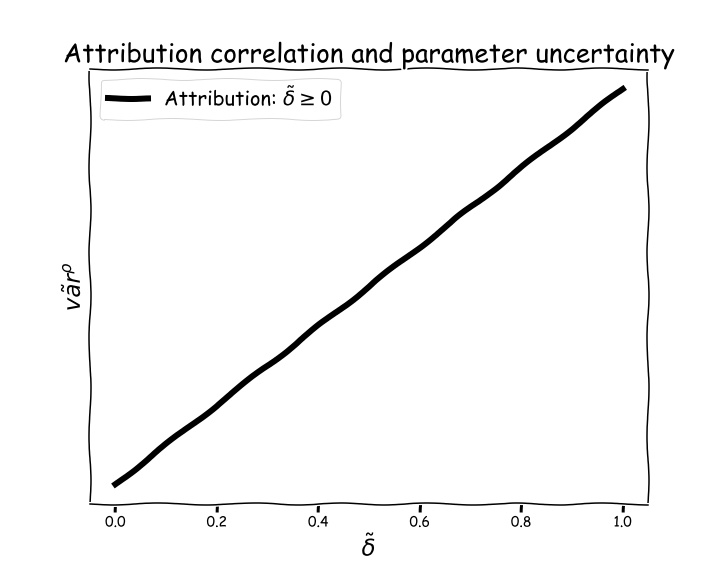
\includegraphics[width=0.7\textwidth]{figures/corr_var.jpg}
	\end{figure}
\end{frame}


\begin{frame}{Prediction 2. extrapolation of experienced volatility into perceived risks}
	\begin{figure}
		\centering 
		\label{var_experience_var}
		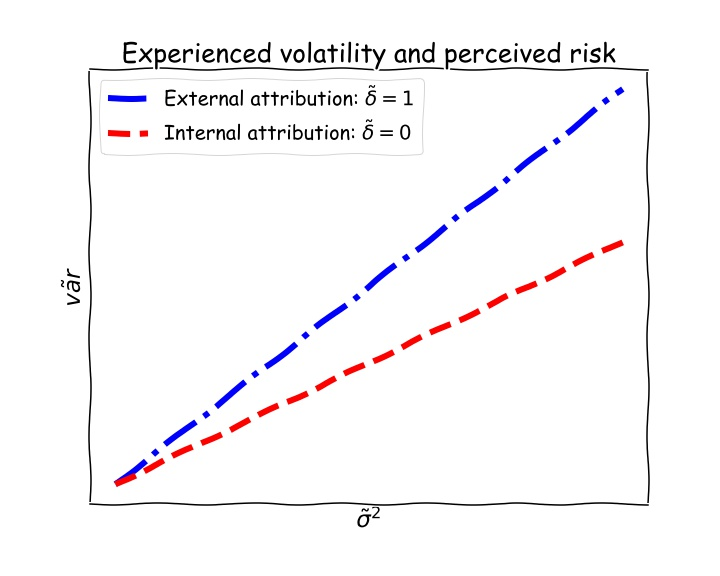
\includegraphics[width=0.7\textwidth]{figures/var_experience_var.jpg}
	\end{figure}
\end{frame}

\begin{frame}{Attribution errors}
	\begin{itemize}
		\item positive (negative) shock $\rightarrow$ internal (external) attribution
	\end{itemize}
	\begin{eqnarray}
		\begin{split}
			\textcolor{blue}{\text{Attribution function:}} \quad \tilde \delta(\Delta y_{i,t}) = 1- \frac{1}{(1+e^{\alpha-\theta\Delta y_{i,t}})}
		\end{split}
	\end{eqnarray}
	\begin{itemize}
		\item $\theta$: degree of attribution error
		\item $\alpha$: unbiasedness of attribution
	\end{itemize}
	
\begin{figure}
	\centering 
	\label{var_experience_var}
	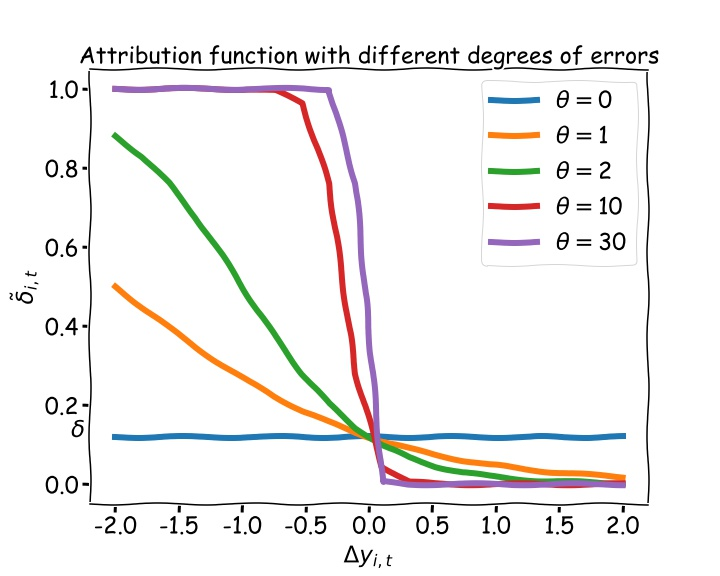
\includegraphics[width=0.4\textwidth]{figures/theta_corr.jpg}
\end{figure}
\end{frame}

\begin{frame}{Prediction 3. \textcolor{red}{Counter-cylical} perceived risks under aggregate risk and attribution error}
	\begin{eqnarray}
		\begin{split}
			\tilde {Var}_{t}(\Delta y_{i,t+1}) & = \underbrace{\lambda_t}_{\text{lucky fraction}} \tilde{Var_t}^{internal} + (1-\lambda_t) \tilde{Var_t}^{external} 
		\end{split}
	\end{eqnarray}
	\begin{itemize} 
		\item Aggregate  versus idionsyncratic risks
		\begin{itemize}
			\item Aggregate: $\lambda_t$ is procyclical.   
			\item Idionsyncratic: $\lambda_t \approx 0.5$ 
		\end{itemize}
		\item With and without attribution errors
		\begin{itemize}
			\item Attribution error: $\tilde{Var_t}^{external} >\tilde{Var_t}^{internal}$ 
			\item No error: $\tilde{Var_t}^{external} =\tilde{Var_t}^{internal}$
		\end{itemize}
	\end{itemize}
	
\end{frame}


%\begin{frame}{\textcolor{red}{Counter-cyclical} perceived risks, continued}
%		\begin{figure}
%		\centering 
%		\label{var_experience_var}
%		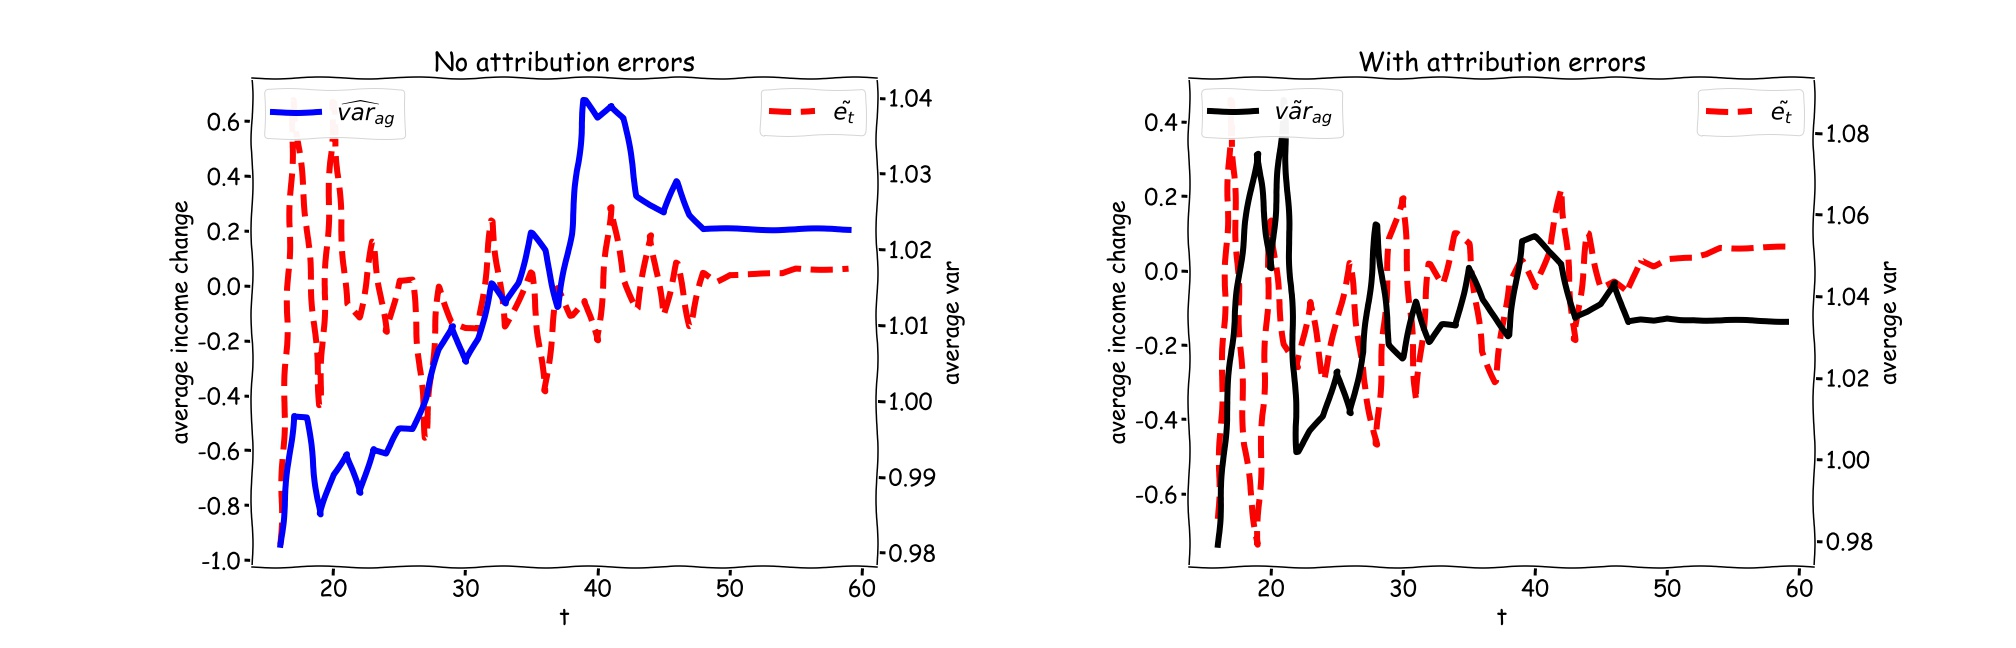
\includegraphics[width=\textwidth]{figures/var_recent_change_sim.jpg}
%	\end{figure}
%	\begin{figure}
%		\centering 
%		\label{var_experience_var}
%		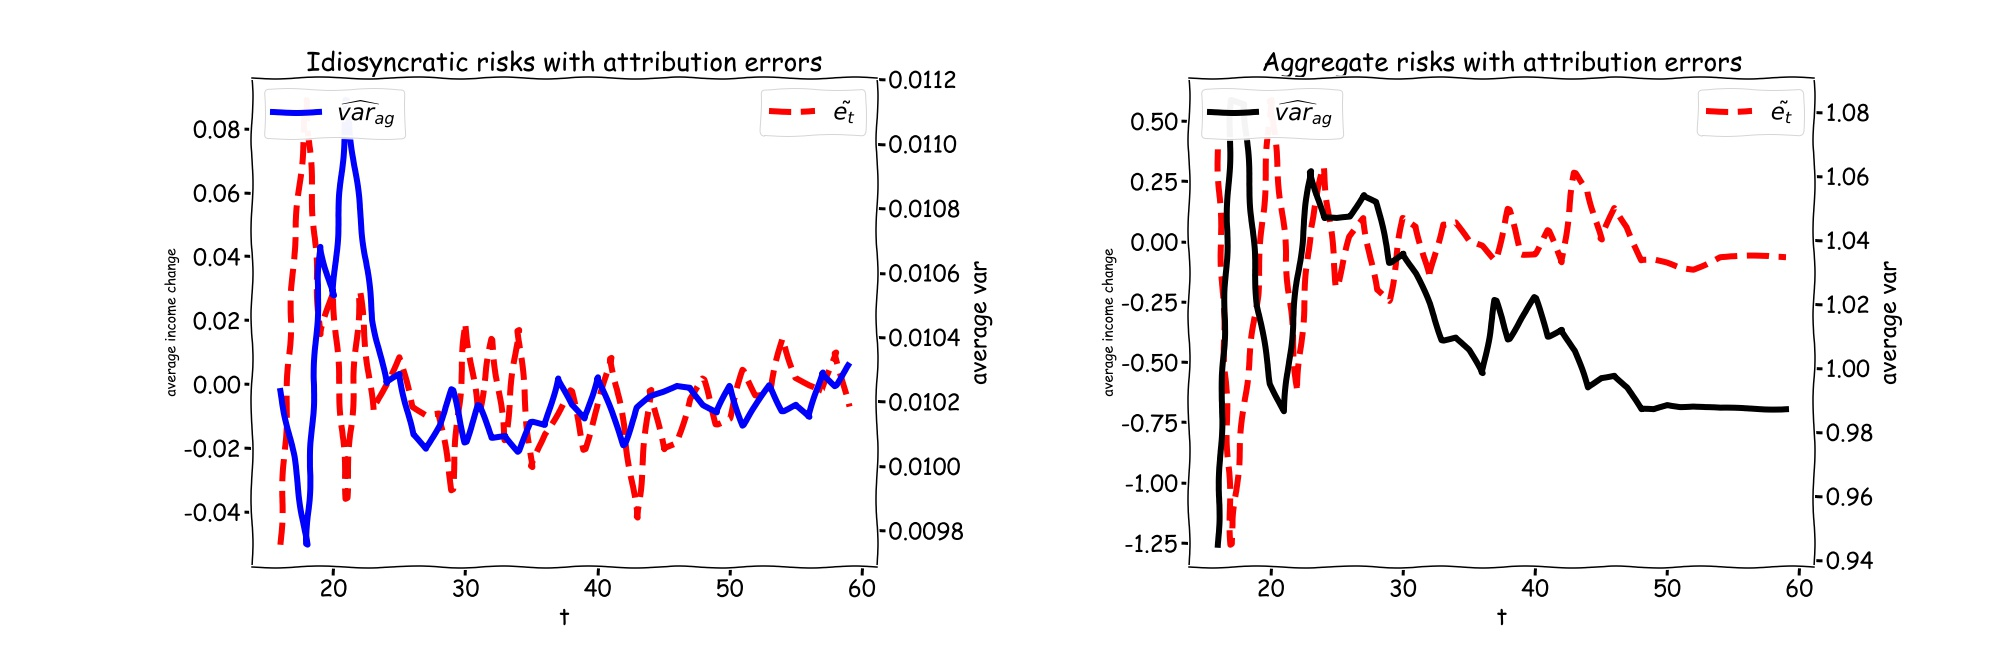
\includegraphics[width=\textwidth]{figures/var_recent_change_sim2.jpg}
%	\end{figure}
%\end{frame}


%\begin{frame}{Prediction 4. perceived risk declines over age}
%	\begin{figure}
%		\centering 
%		\label{var_experience_var}
%		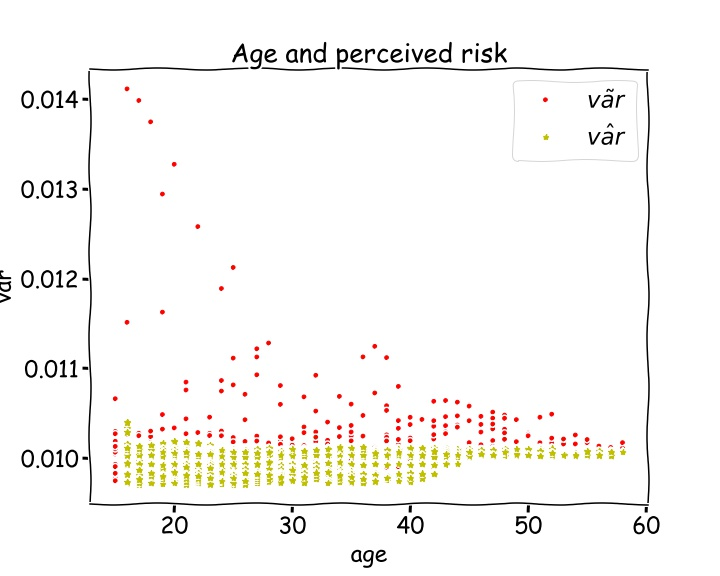
\includegraphics[width=0.7\textwidth]{figures/var_age_sim.jpg}
%	\end{figure}
%\end{frame}


%\begin{frame}{Prediction 3. skewed U-shaped income profile}
%	\begin{eqnarray}
%		\begin{split}
%			\tilde {Var}_{i,t}(\Delta y_{i,t+1})  = [(\sum^{t-c}_{k=0}\sum^{n}_{j=1}y^2_{j,t-k-1})^{-1}(1+\tilde\delta_{i,t}(n-1))y^2_{i,t} + 1] s^2_{i,t} 
%		\end{split}
%	\end{eqnarray}
%		\begin{figure}
%		\centering 
%		\label{var_experience_var}
%		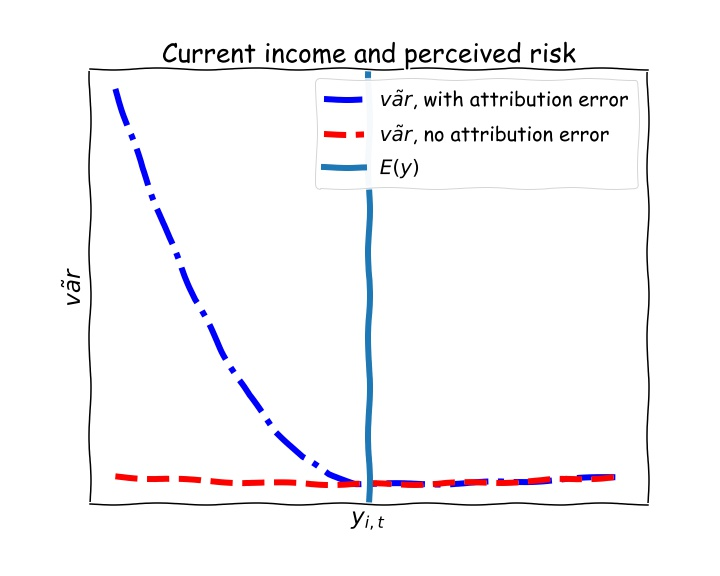
\includegraphics[width=0.6\textwidth, height = 0.6\textheight]{figures/var_recent.jpg}
%	\end{figure}
%\end{frame}



%\subsection{Simulation}	


%\begin{frame}{Simulated income profile}
%	\begin{figure}
%		\centering 
%		\label{var_experience_var}
%		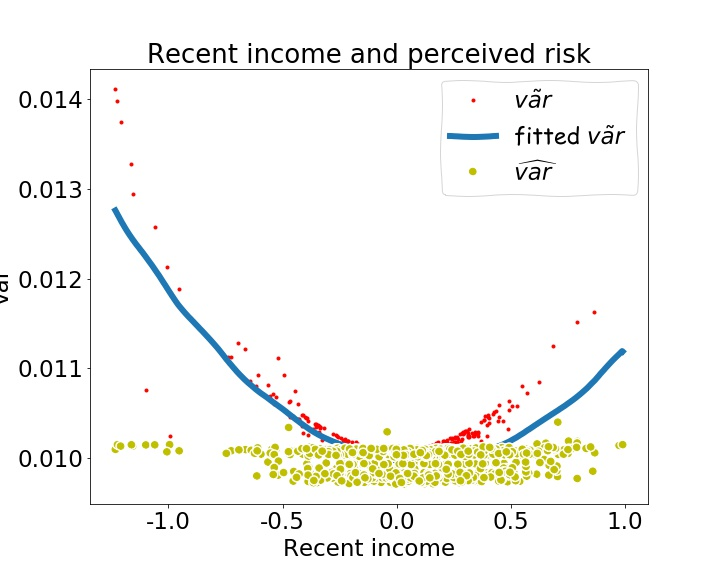
\includegraphics[width=0.7\textwidth]{figures/var_recent_sim.jpg}
%	\end{figure}
%\end{frame}



%\begin{frame}{Robustness}
%	\begin{itemize}
%		\item Permanent and transitory income risk 
%		\item Serial correlation 
%		\item Time-varying income risks 
%		\item More regressors 
%	\end{itemize}
%\end{frame}



\section{Empirical facts}


%\begin{frame}{Data}
%	\begin{table}
%		\centering
%		\caption{Survey of Consumer Expectations}
%		\label{SCE_data_sum}
%		\adjustbox{max height=0.5\textheight, max width=\textwidth}{ 
%			\begin{tabular}{lll}
%				\hline 
%				Time period                                    & 2013M6-2019M6           \\
%				Frequency                                      & monthly                                 \\
%				Sample size                                    & 1,300                                  \\
%				Density variable                    &  \textcolor{blue}{1-yr-ahead earning growth   (same position/hours) }           \\
%				Pannel structure                               & 12 months      \\
%				Demographics                     & educ, income, age, gender, state       \\
%				\hline 
%			\end{tabular}
%		}
%	\end{table}
%	\begin{itemize}
%		\item density estimation following \cite{engelberg_comparing_2009}
%		\item exclude top and bottom 1\% values of each moment
%	\end{itemize}
%\end{frame}


%\begin{frame}{Definition}
%	\begin{itemize}
%		\item $\Delta Y_{i,t+12}$ : the next-year income growth of the same job/position/hours, seperate from unemployement risk
%		\item Moments of interest 
%		\begin{itemize}
%			\item expected growth, $\text{exp}_{i,t} = E_{i,t} (\Delta Y_{i,t+12})$
%			\item variance: $\overline {var}_{i,t}(\Delta Y_{i,t+12})$ 
%			\item iqr: $\overline {iqr}_{i,t}(\Delta Y_{i,t+12})$ 
%			\item skewness: $\overline {skew}_{i,t}(\Delta Y_{i,t+12})$
%		\end{itemize}
%		\item Nominal and real income growth 
%		\begin{itemize}
%			\item $\text{rexp}_{i,t} =E_{i,t}(\Delta Y^r_{i,t+12}) =E_i(\Delta Y_{i,t+12}^n) - E_{i,t+12}(\pi_{t+12})$
%			\item $\overline{rvar}_{i,t}=\overline {var}_{i,t}(\Delta Y_{i,t+12}^n) +  \overline {var}_{i,t}(\pi_{t+12})$
%		\end{itemize}
		%\item Does not reflect unemployment risk 
		%\begin{itemize}
		%	\item Can be converted into the unconditional risk using perceived unemployment risk ( same-job-hour risk is just a lower bound).  %% I did not do the adjustment. I use same-job-hour income growth throughout my analysis.
		%\end{itemize}
%	\end{itemize}
%\end{frame}

\subsection{Cross-sectional patterns}

%%% the purpose of examining cross-sectional distribution are twofold. First, since there is not much work that has been showing these basic facts. I think it is important to be aware of new facts. Second, for those of you who are still a little doubtful about the survey data, it helps us assure the surveyed data shows some patterns that are intuitive and consistent.  

%\begin{frame}{Cross-sectional of income growth expectation}
%	\begin{figure}
%		\centering
%		\label{incexp_hist}
%		\begin{subfigure}[b]{0.45\textwidth}
%			\centering
%			\caption{expected growth of nominal}
%			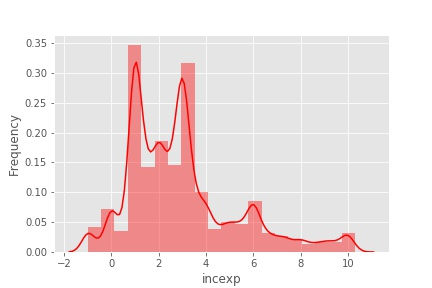
\includegraphics[width=\textwidth]{figures/hist_incexp}
%		\end{subfigure}
%		\begin{subfigure}[b]{0.45\textwidth}
%			\centering
%			\caption{expected growth of real}
%			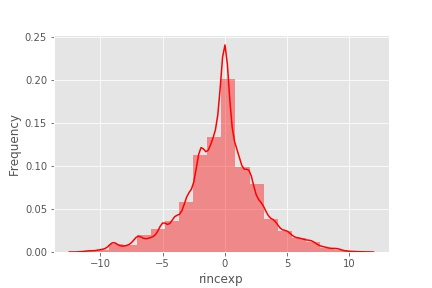
\includegraphics[width=\textwidth]{figures/hist_rincexp}
%		\end{subfigure}
%	\end{figure}
%	\begin{itemize}
%		\item nominal income: right-skewed and mostly positive   
%		\item real income: symmetric around zero  
%	\end{itemize}
%\end{frame}

%\begin{frame}{Cross-section of income risks}
%	\begin{figure}
%		\centering
%		\label{incvar_hist}
%			\begin{subfigure}[b]{0.45\textwidth}
%			\centering
%			\caption{nominal income risk}
%		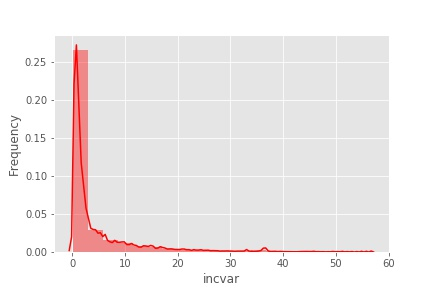
\includegraphics[width=\textwidth]{figures/hist_incvar}
%		\end{subfigure}
%		\begin{subfigure}[b]{0.45\textwidth}
%		\centering
%		\caption{real income risk}
%		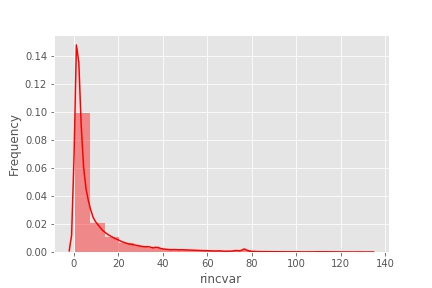
\includegraphics[width=\textwidth]{figures/hist_rincvar}
%	\end{subfigure}
%	\end{figure}
%	\begin{itemize}
%		\item average:  $2.5\%$ standard deviation for nominal and $3.5\%$ standard deviation for real income
		%\item just a lower bound: before adjustment of unemployment risk 
%	\end{itemize}
%\end{frame}


%\begin{frame}{Perceived income risks by household income}
%	\begin{figure}[ht]
%		\label{ts_incvar_HHinc_g_mean}
%		\begin{subfigure}[b]{0.7\textwidth}
%			\centering
%			\caption{income risks}
%			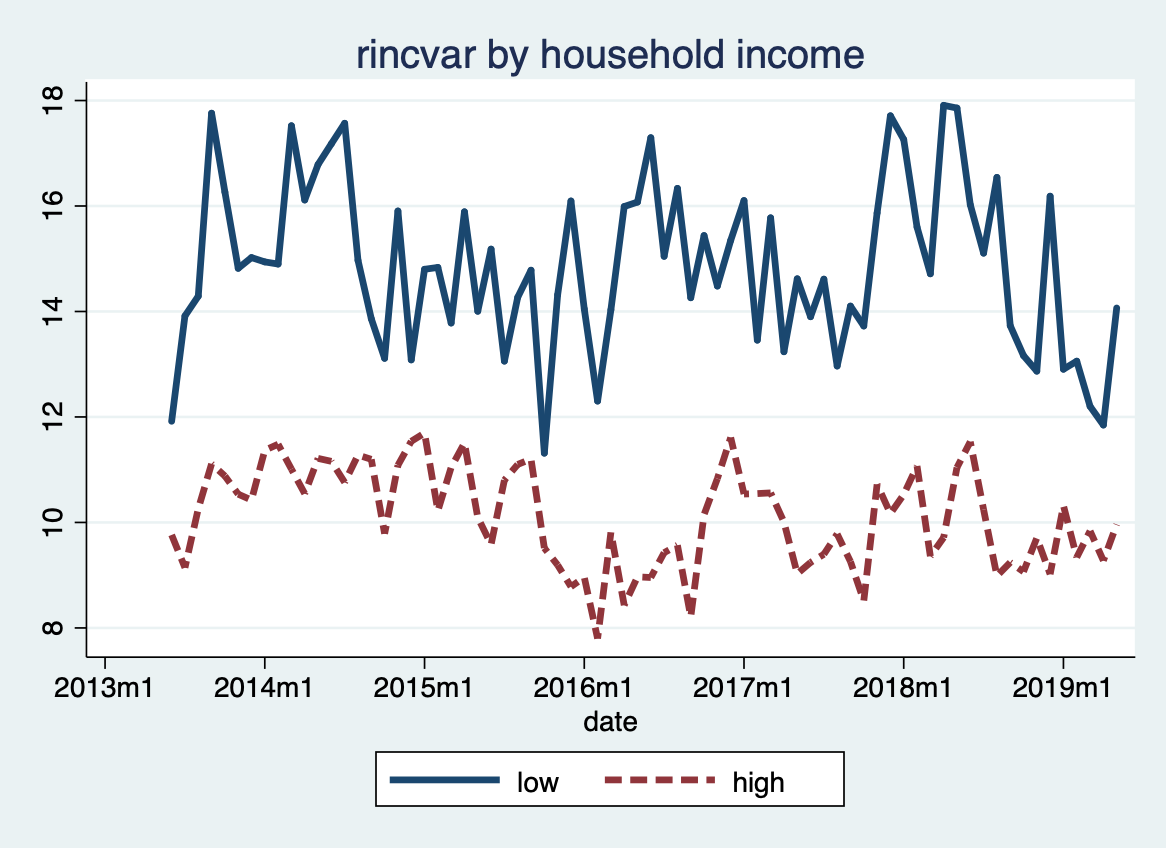
\includegraphics[width=\textwidth, height = 0.33\textheight]{figures/ts_rincvar_HHinc_g_mean.png}
%		\end{subfigure}
%		\begin{subfigure}[b]{0.7\textwidth}
%			\caption{skewness}
%			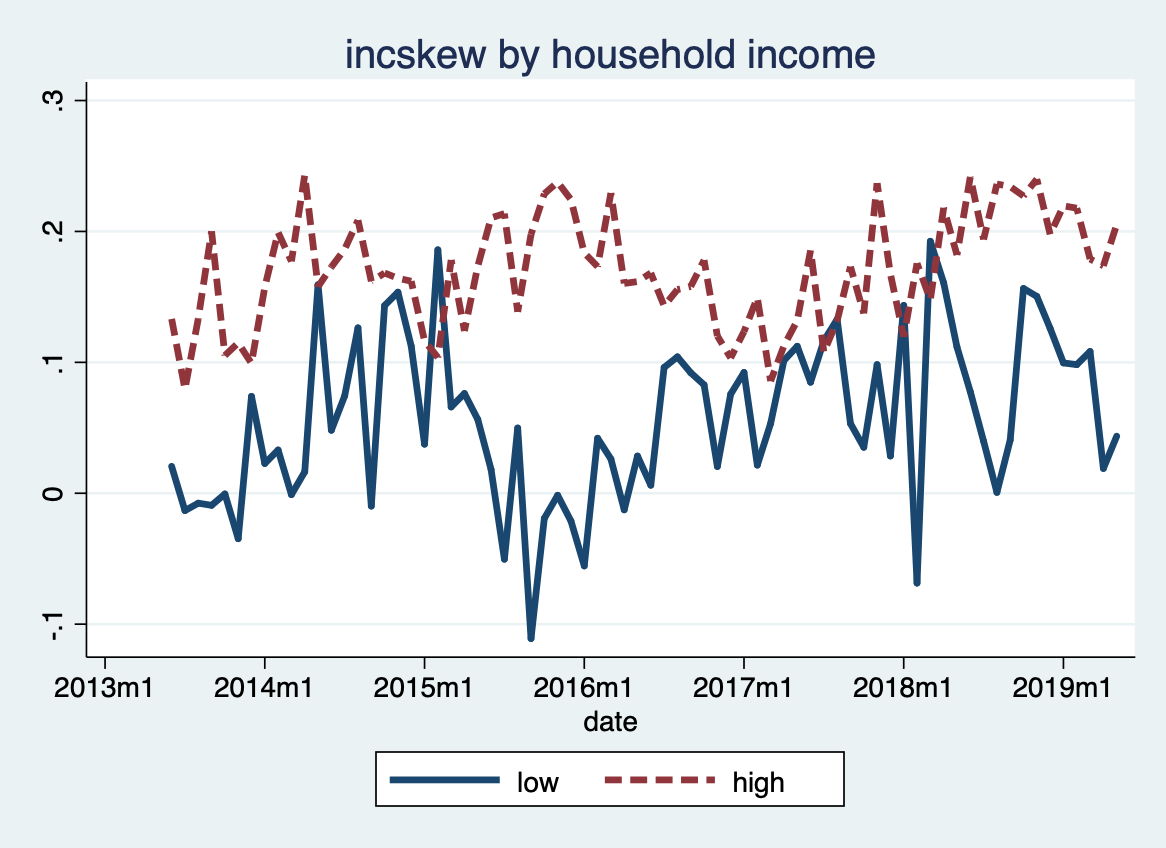
\includegraphics[width=\textwidth, height = 0.33\textheight]{figures/ts_incskew_HHinc_g_mean.png}
%		\end{subfigure}
%	\end{figure}
%\end{frame}


\begin{frame}{Perceived risks by household income}
\begin{figure}
	\centering
	\label{boxplot_hhinc}
	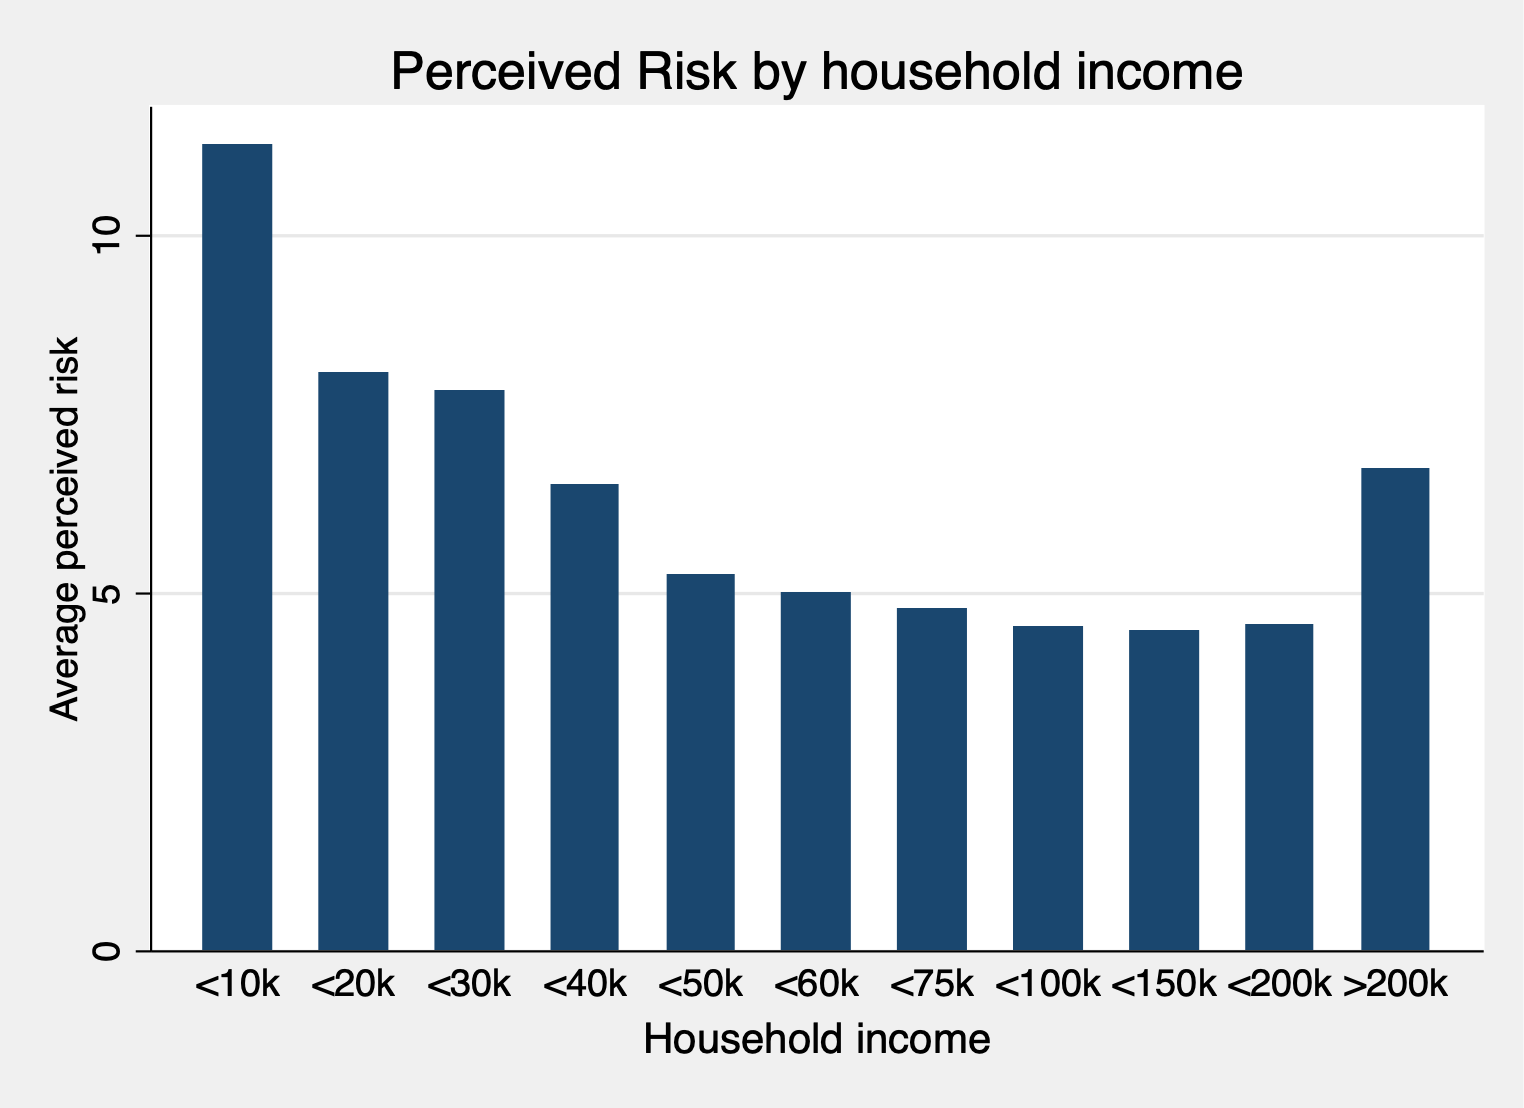
\includegraphics[width=0.7\textwidth]{figures/boxplot_var_HHinc_stata}
\end{figure}
	%\begin{itemize}
	%\item Similar to the pattern of earning growth dispersion conditional on income in \cite{bloom2018great}. 
%\end{itemize}
\end{frame}

\begin{frame}{Perceived risks by age}
	\begin{figure}[ht]
		%\caption{Perceived Risk} 
		\label{ts_incvar_age_g_mean}
		\centering
		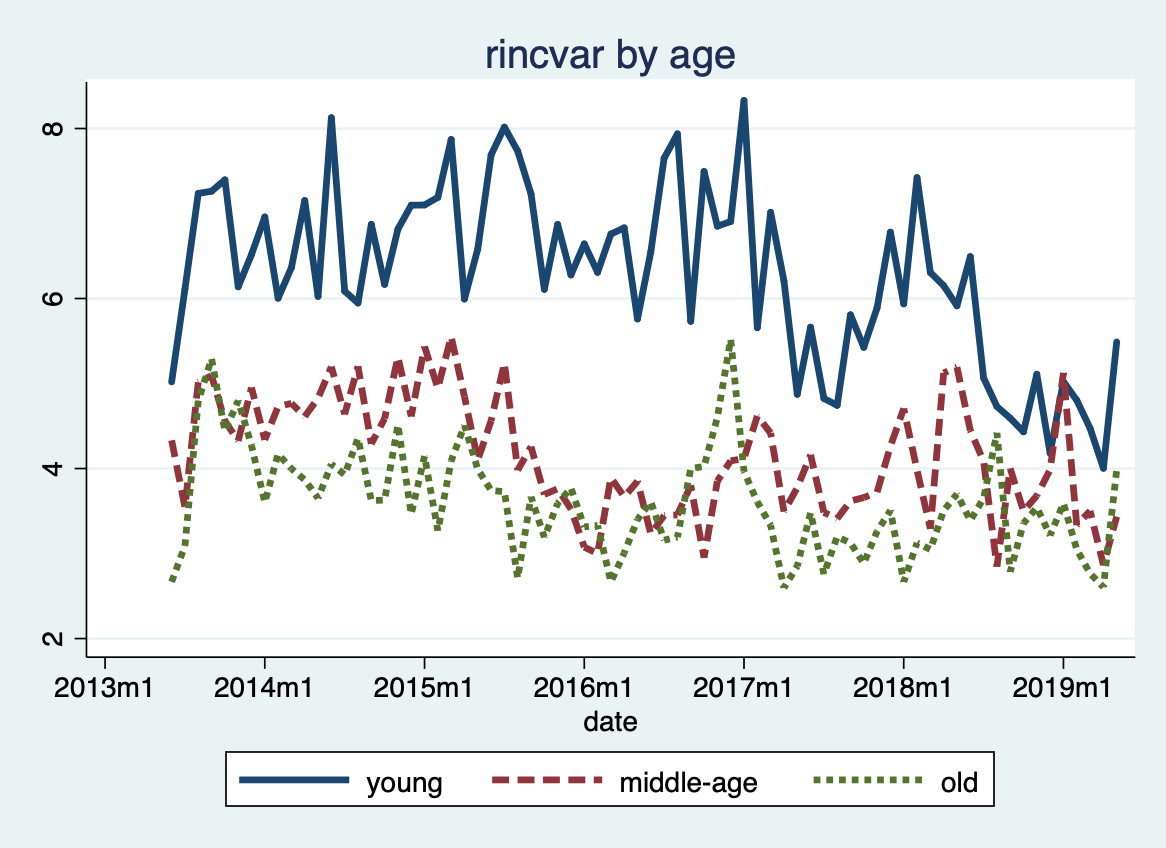
\includegraphics[width=0.7\textwidth]{figures/ts_rincvar_age_g_median.png}
		%	\begin{subfigure}[b]{0.46\textwidth}
		%			\caption{skewness}
		%			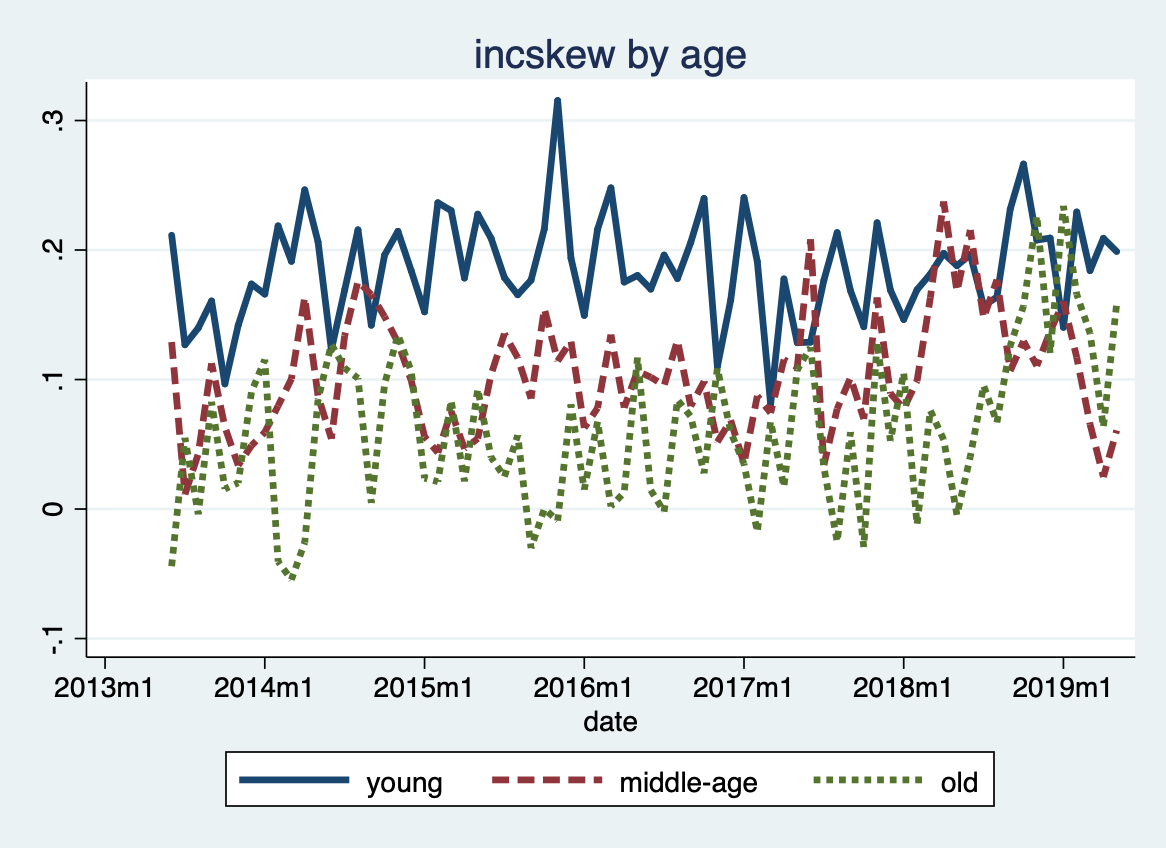
\includegraphics[width=\textwidth, height = 0.33\textheight]{figures/ts_incskew_age_g_mean.png}
		%	\end{subfigure}
	\end{figure}
	%\begin{itemize}
	%	\item in line with existing findings, for instance  
	%	\cite{bloom2018great}. 
	%\end{itemize}
\end{frame}

%\begin{frame}{Perceived income risks by age}
%	\begin{figure}
%		\centering
%		\label{boxplot_age_gr}
%		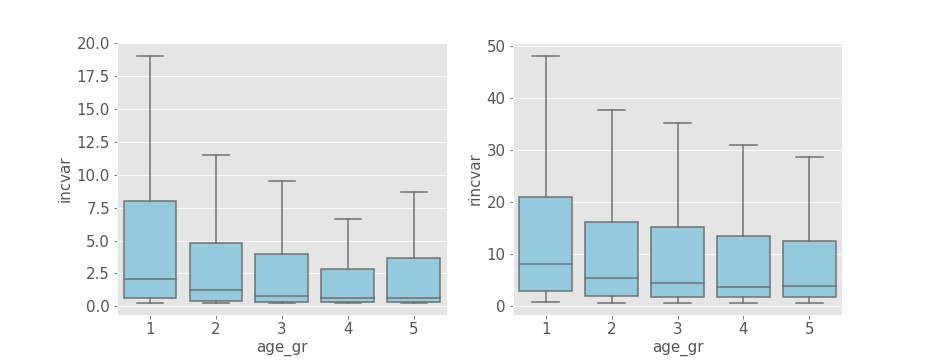
\includegraphics[width=0.8\textwidth]{figures/boxplot_exp_age_gr} \\
%		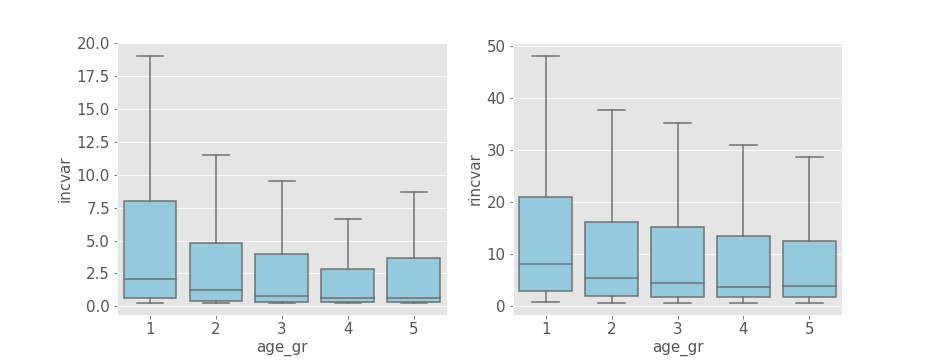
\includegraphics[width=0.8\textwidth]{figures/boxplot_var_age_gr}
%	\end{figure}
%	\begin{itemize}
%		\item 
%	\end{itemize}
%\end{frame}

\begin{frame}{Perceived risks and experience}
	\begin{itemize}
		\item Approximated experienced volatility: $s^2_{c,t}$, MSE of the income regression for the PSID sample between $c$ and $t$ 
		\item Perceived risk: $\overline{var_{c,t}}$: average across individuals within cohort $c$ at time $t$
	\end{itemize}
	\begin{figure}[ht]
		%\caption{Perceived risk and experienced volatility}
		\label{ts_incvar_byear_g_mean}
		\centering
		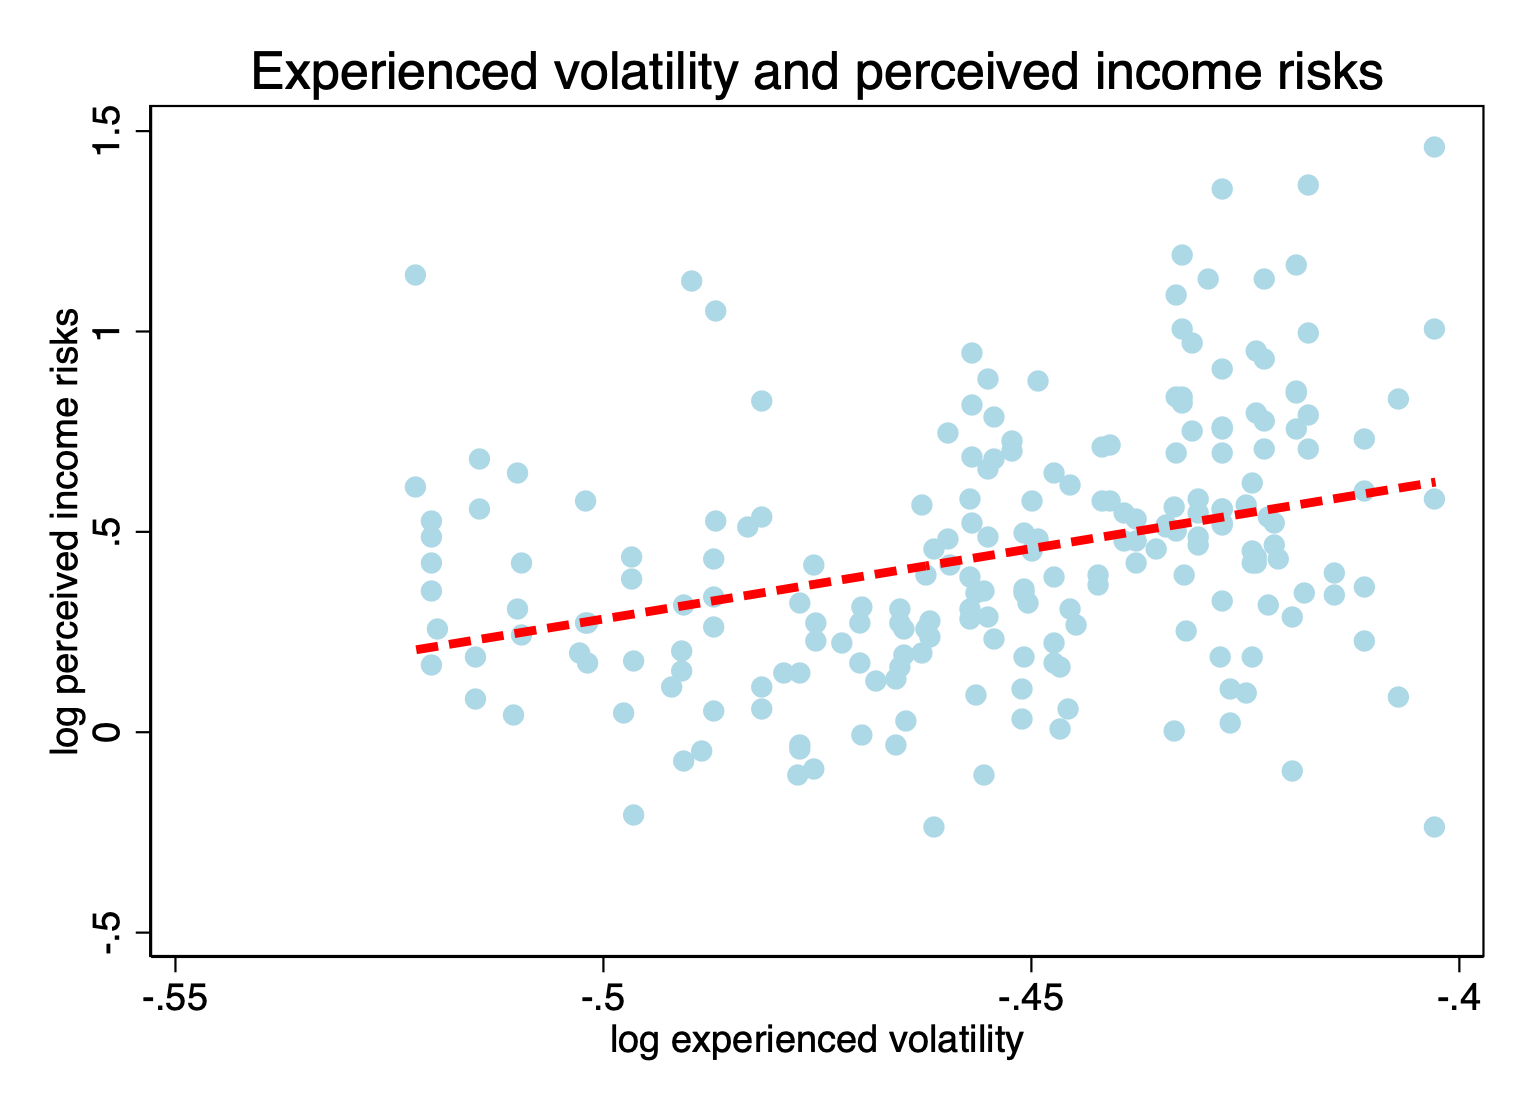
\includegraphics[width=0.6\textwidth]{figures/experience_var_var_data.png}
		%		\begin{subfigure}[b]{0.46\textwidth}
		%			\caption{skewness}
		%			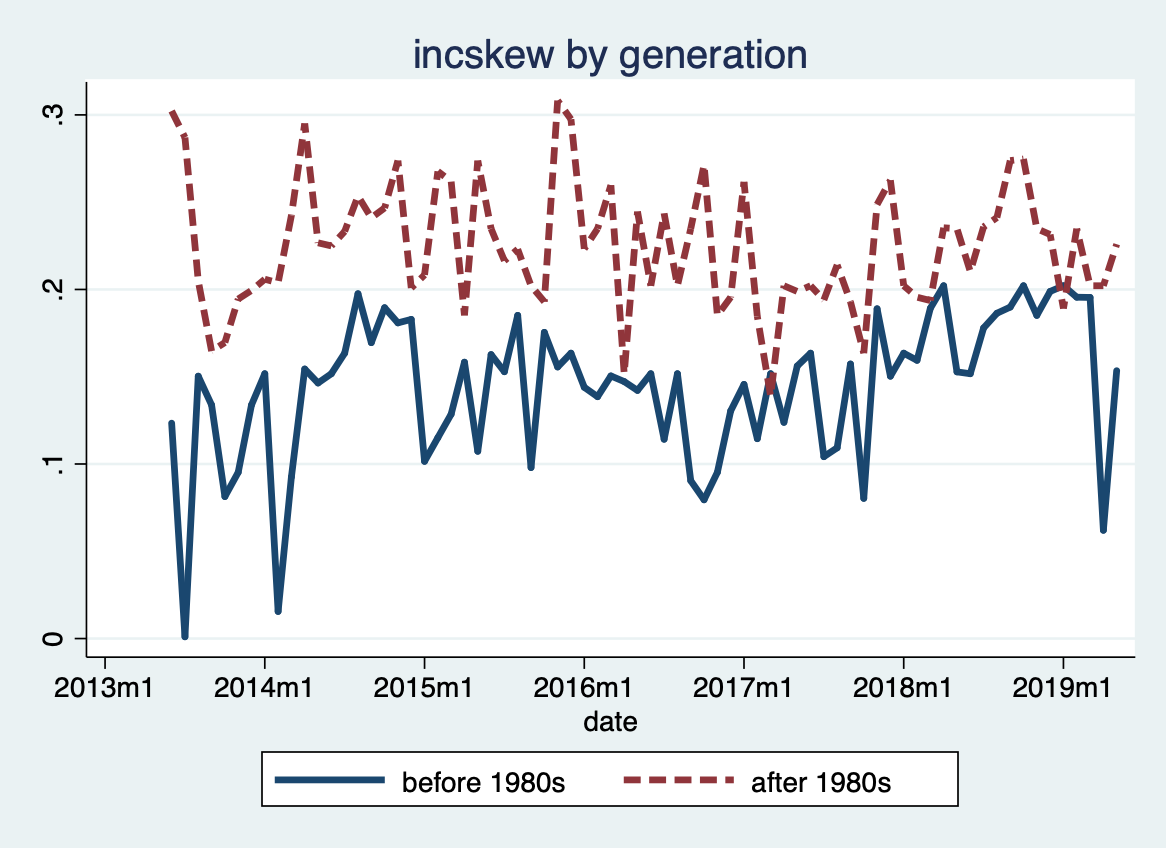
\includegraphics[width=\textwidth, height = 0.33\textheight]{figures/ts_incskew_byear_g_median.png}
		%		\end{subfigure}
	\end{figure}
\end{frame}


\begin{frame}{Perceived risks and experienced volatility}
	\begin{eqnarray*}
		\underbrace{log(\overline{\text{var}}_{i,c,t})}_{\text{log perceived risk}} = a + \textcolor{red}{\zeta} \underbrace{log(\hat s^2_{c,t})}_{\text{log experienced volatility}}+ Z\underbrace{\Gamma_{i,t}}_{\text{individual controls}} + \xi_{i,t}
	\end{eqnarray*}
	
	\begin{table}
		\centering
		%\caption{Correlation between Perceived Income Risks and Stock Market Return}
		\label{micr_corr_history_vol}
		\adjustbox{max height=0.5\textheight, max width=\textwidth}{ 
			\begin{tabular}{lllllll}
				& Perceived risk & Perceived risk & Perceived risk & Perceived iqr & Perceived iqr & Perceived iqr \\
				\hline
				log experienced volatility & 1.291**        & 1.265**        & 1.208**        & 0.690**       & 0.713**       & 0.650**       \\
				& (3.08)         & (3.02)         & (2.61)         & (3.05)        & (3.16)        & (2.62)        \\
				&                &                &                &               &               &               \\
				\hline
				R-squre                    & 0.0170         & 0.0222         & 0.0243         & 0.0118        & 0.0168        & 0.0269        \\
				N                          & 40158          & 40158          & 33485          & 44454         & 44454         & 37058         \\
				Control age                & Yes            & Yes            & Yes            & Yes           & Yes           & Yes           \\
				Control educ               & No             & Yes            & Yes            & No            & Yes           & Yes           \\
				Control income             & No             & No             & Yes            & No            & No            & Yes          \\
				\hline
			\end{tabular}
		}
	\end{table}
	
\end{frame}


%\begin{frame}{Perceived income risks by generation}
%	\begin{figure}
%		\centering
	%	\label{boxplot_byear_gr}
%	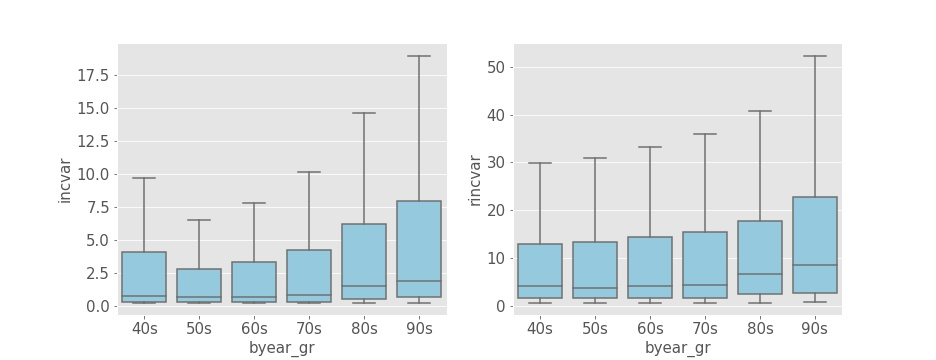
\includegraphics[width=0.8\textwidth]{figures/boxplot_var_byear_gr}
%	\end{figure}
%	\begin{itemize}
	%	\item 
%	\5end{itemize}
%\end{frame}



%\begin{frame}{Perceived income risks by education}
%	\begin{figure}
%		\centering
%		\label{boxplot_educ_gr}
%		\includegraphics[width=0.8\textwidth]{figures/boxplot_exp_edu_gr} \\
%		\includegraphics[width=0.8\textwidth]{figures/boxplot_var_edu_gr}
%	\end{figure}
%	\begin{itemize}
%		\item 
%	\end{itemize}
% \end{frame}



%\begin{frame}{Covariants of perceived risks}
%	\begin{table}
%	\centering
%		\caption{Perceived income risks and individual characteristics}
%		\label{micro_reg}
%		\adjustbox{max height=0.5\textheight, max width=\textwidth}{ 
%\begin{tabular}{ccccccccc}
%	\hline 
%	{} & incvar I & incvar II & incvar III & incvar IIII & rincvar I & rincvar II & rincvar III & rincvar IIII \\
%	\hline 
%	HHinc\_gr=low inc &          &           &    1.56*** &             &           &            &     7.01*** &              \\
%	&          &           &     (0.10) &             &           &            &      (0.19) &              \\
%	educ\_gr=low educ &          &           &            &     0.40*** &           &            &             &      3.82*** \\
%	&          &           &            &      (0.11) &           &            &             &       (0.21) \\
%	gender=male      &          &           &            &    -0.80*** &           &            &             &      2.76*** \\
%	&          &           &            &      (0.10) &           &            &             &       (0.19) \\
%	parttime=yes     &     0.05 &     0.24* &      -0.12 &             &   1.41*** &    1.81*** &        0.19 &              \\
%	&   (0.12) &    (0.13) &     (0.13) &             &    (0.23) &     (0.26) &      (0.26) &              \\
%	selfemp=yes      &  7.21*** &  -0.00*** &   -0.00*** &             &   6.27*** &   -0.00*** &     0.00*** &              \\
%	&   (0.15) &    (0.00) &     (0.00) &             &    (0.27) &     (0.00) &      (0.00) &              \\
%	UEprobAgg        &          &    0.01** &      0.00* &             &           &    0.05*** &     0.04*** &              \\
%	&          &    (0.00) &     (0.00) &             &           &     (0.00) &      (0.00) &              \\
%	UEprobInd        &          &   0.03*** &    0.02*** &             &           &    0.05*** &     0.04*** &              \\
%	&          &    (0.00) &     (0.00) &             &           &     (0.00) &      (0.00) &              \\
%	Intercept        &  4.64*** &   3.75*** &    3.28*** &     5.72*** &  12.42*** &   12.21*** &    10.16*** &     11.16*** \\
%	&   (0.05) &    (0.12) &     (0.12) &      (0.07) &    (0.10) &     (0.24) &      (0.25) &       (0.14) \\
%	\hline 
%	N                &    54029 &     47331 &      47331 &       47457 &     50730 &      44382 &       44382 &        44517 \\
%	R2               &     0.05 &      0.00 &       0.01 &        0.00 &      0.01 &       0.01 &        0.04 &         0.01 \\
%	\hline 
%\end{tabular}
%}
%	\end{table}
%end{frame}


%\subsection{Perceived risks and decisions}


%\begin{frame}{Perveived risks and household spending}
	
%\begin{eqnarray*}
%	E_{i,t} (\Delta C_{i,t+12}) = u_0 + u_1 \overline{\text{risks}}_{i,t} (\Delta Y_{i,t+12}) + \xi_{i,t}  
%\end{eqnarray*}
%	\begin{table}
%		\centering
		%\caption{Perceived income risks and household spending}
%		\label{spending_reg}
%		\adjustbox{max height=0.5\textheight, max width=\textwidth}{ 
	
%	\begin{tabular}{ccccccll}
%		\hline 
%		{} & spending I & spending II & spending III & spending IIII & spending IIIII & spending IIIIII & spending IIIIIII \\
%		\hline 
%		incexp    &    0.39*** &             &              &               &                &                 &                  \\
%		&     (0.08) &             &              &               &                &                 &                  \\
		
%		rincexp   &            &      -0.04* &              &               &                &                 &                  \\
%		&            &      (0.02) &              &               &                &                 &                  \\
%		incvar    &            &             &      0.07*** &               &                &                 &                  \\
%		&            &             &       (0.02) &               &                &                 &                  \\
%		
%		rincvar   &            &             &              &       0.07*** &                &                 &                  \\
%		&            &             &              &        (0.01) &                &                 &                  \\
%		
%		UEprobAgg &            &             &              &               &                &         0.04*** &                  \\
%		&            &             &              &               &                &          (0.01) &                  \\
%		UEprobInd &            &             &              &               &          -0.01 &                 &                  \\
%		&            &             &              &               &         (0.01) &                 &                  \\
		
%		incskew   &            &             &              &               &                &                 &             0.21 \\
%		&            &             &              &               &                &                 &           (0.43) \\
%		\hline 
%		N         &      55673 &       50997 &        55465 &         52099 &          54315 &           85468 &            55029 \\
%		R2        &       0.00 &        0.00 &         0.00 &          0.00 &           0.00 &            0.00 &             0.00 \\
%		\hline 
%	\end{tabular}
%		}
%	\end{table}
%\begin{itemize}
%	\item  Higher perceived risks $\rightarrow$ higher expected spending growth. 
%\end{itemize}
%\end{frame}

\subsection{Coutercylical perceived risks}

\begin{frame}{Perceived risks and recent (past) wage growth}
	\begin{itemize}
		\item $\overline{\text{var}_{t}} $: average perceived risk across individuals
		\item  $log(\text{wage}_t) - log(\text{wage}_{t-3})$: quarterly growth in average hourly wage
	\end{itemize}
	\begin{figure}
		\centering
		\label{ts_var}
		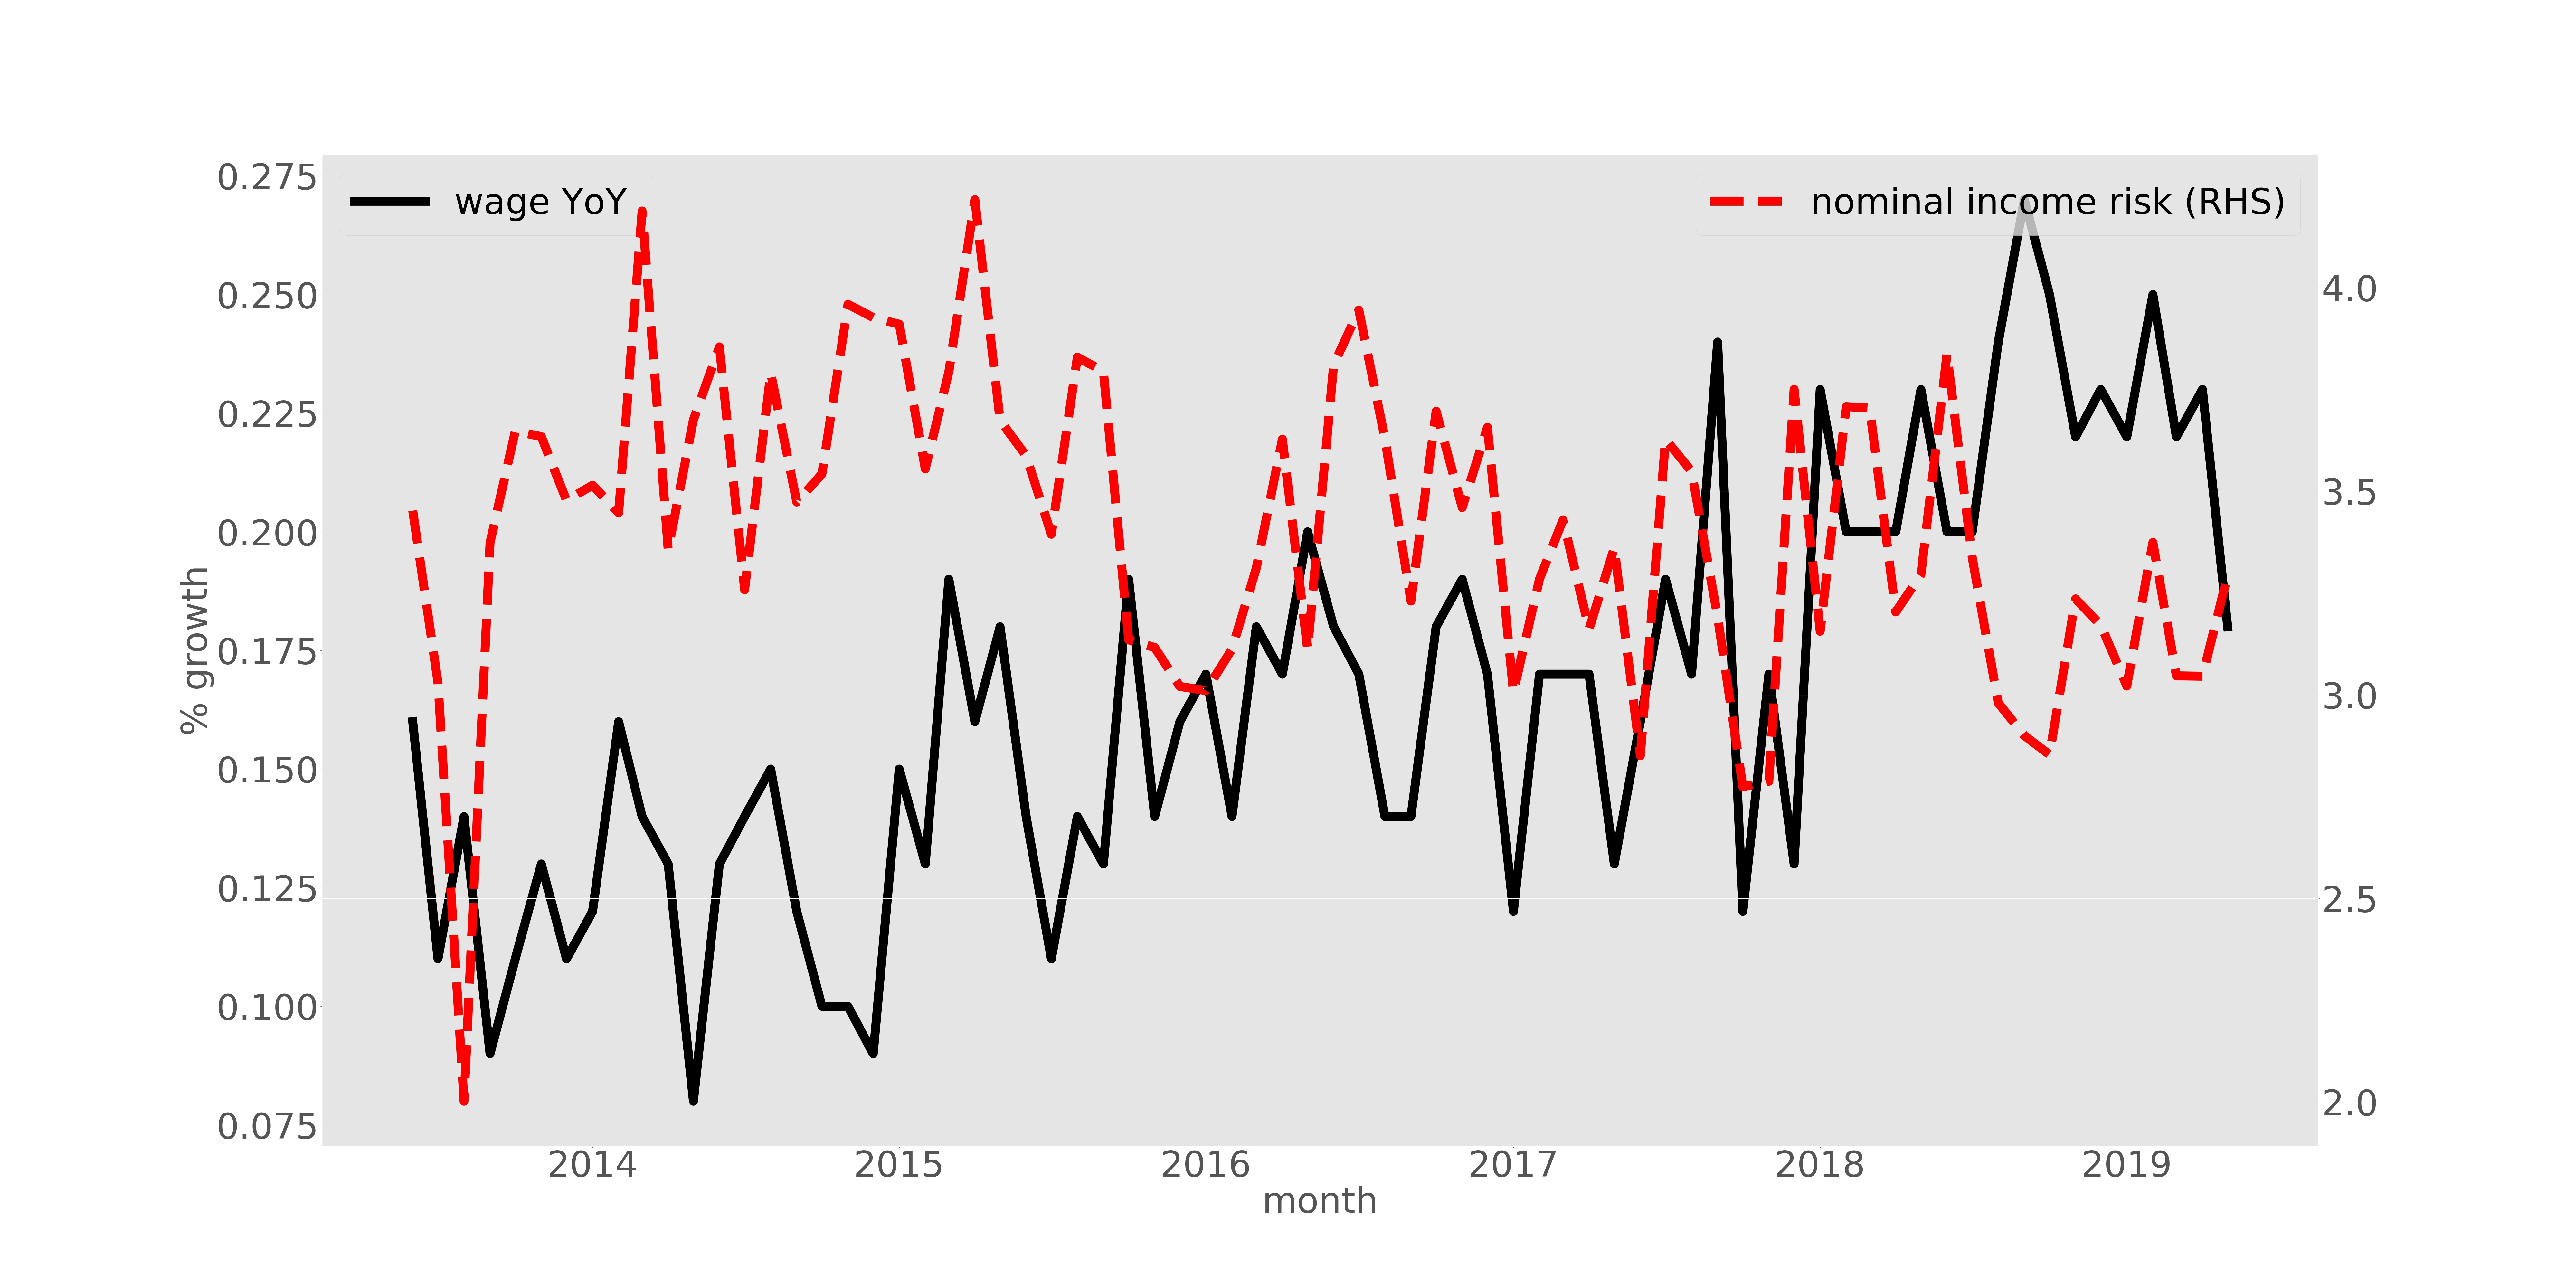
\includegraphics[width=\textwidth]{figures/tsMeanvar_he.jpg}
	\end{figure}
\end{frame}


%\begin{frame}{Perceived \textcolor{blue}{real} income risks and past wage growth}
%	\begin{itemize}
%	\item $\overline{\text{rvar}_{t}} $
%	\item  $log(\text{wage}_t) - log(\text{wage}_{t-3})$
%\end{itemize}
%	\begin{figure}
%		\centering 
%		\label{ts_skew}
%		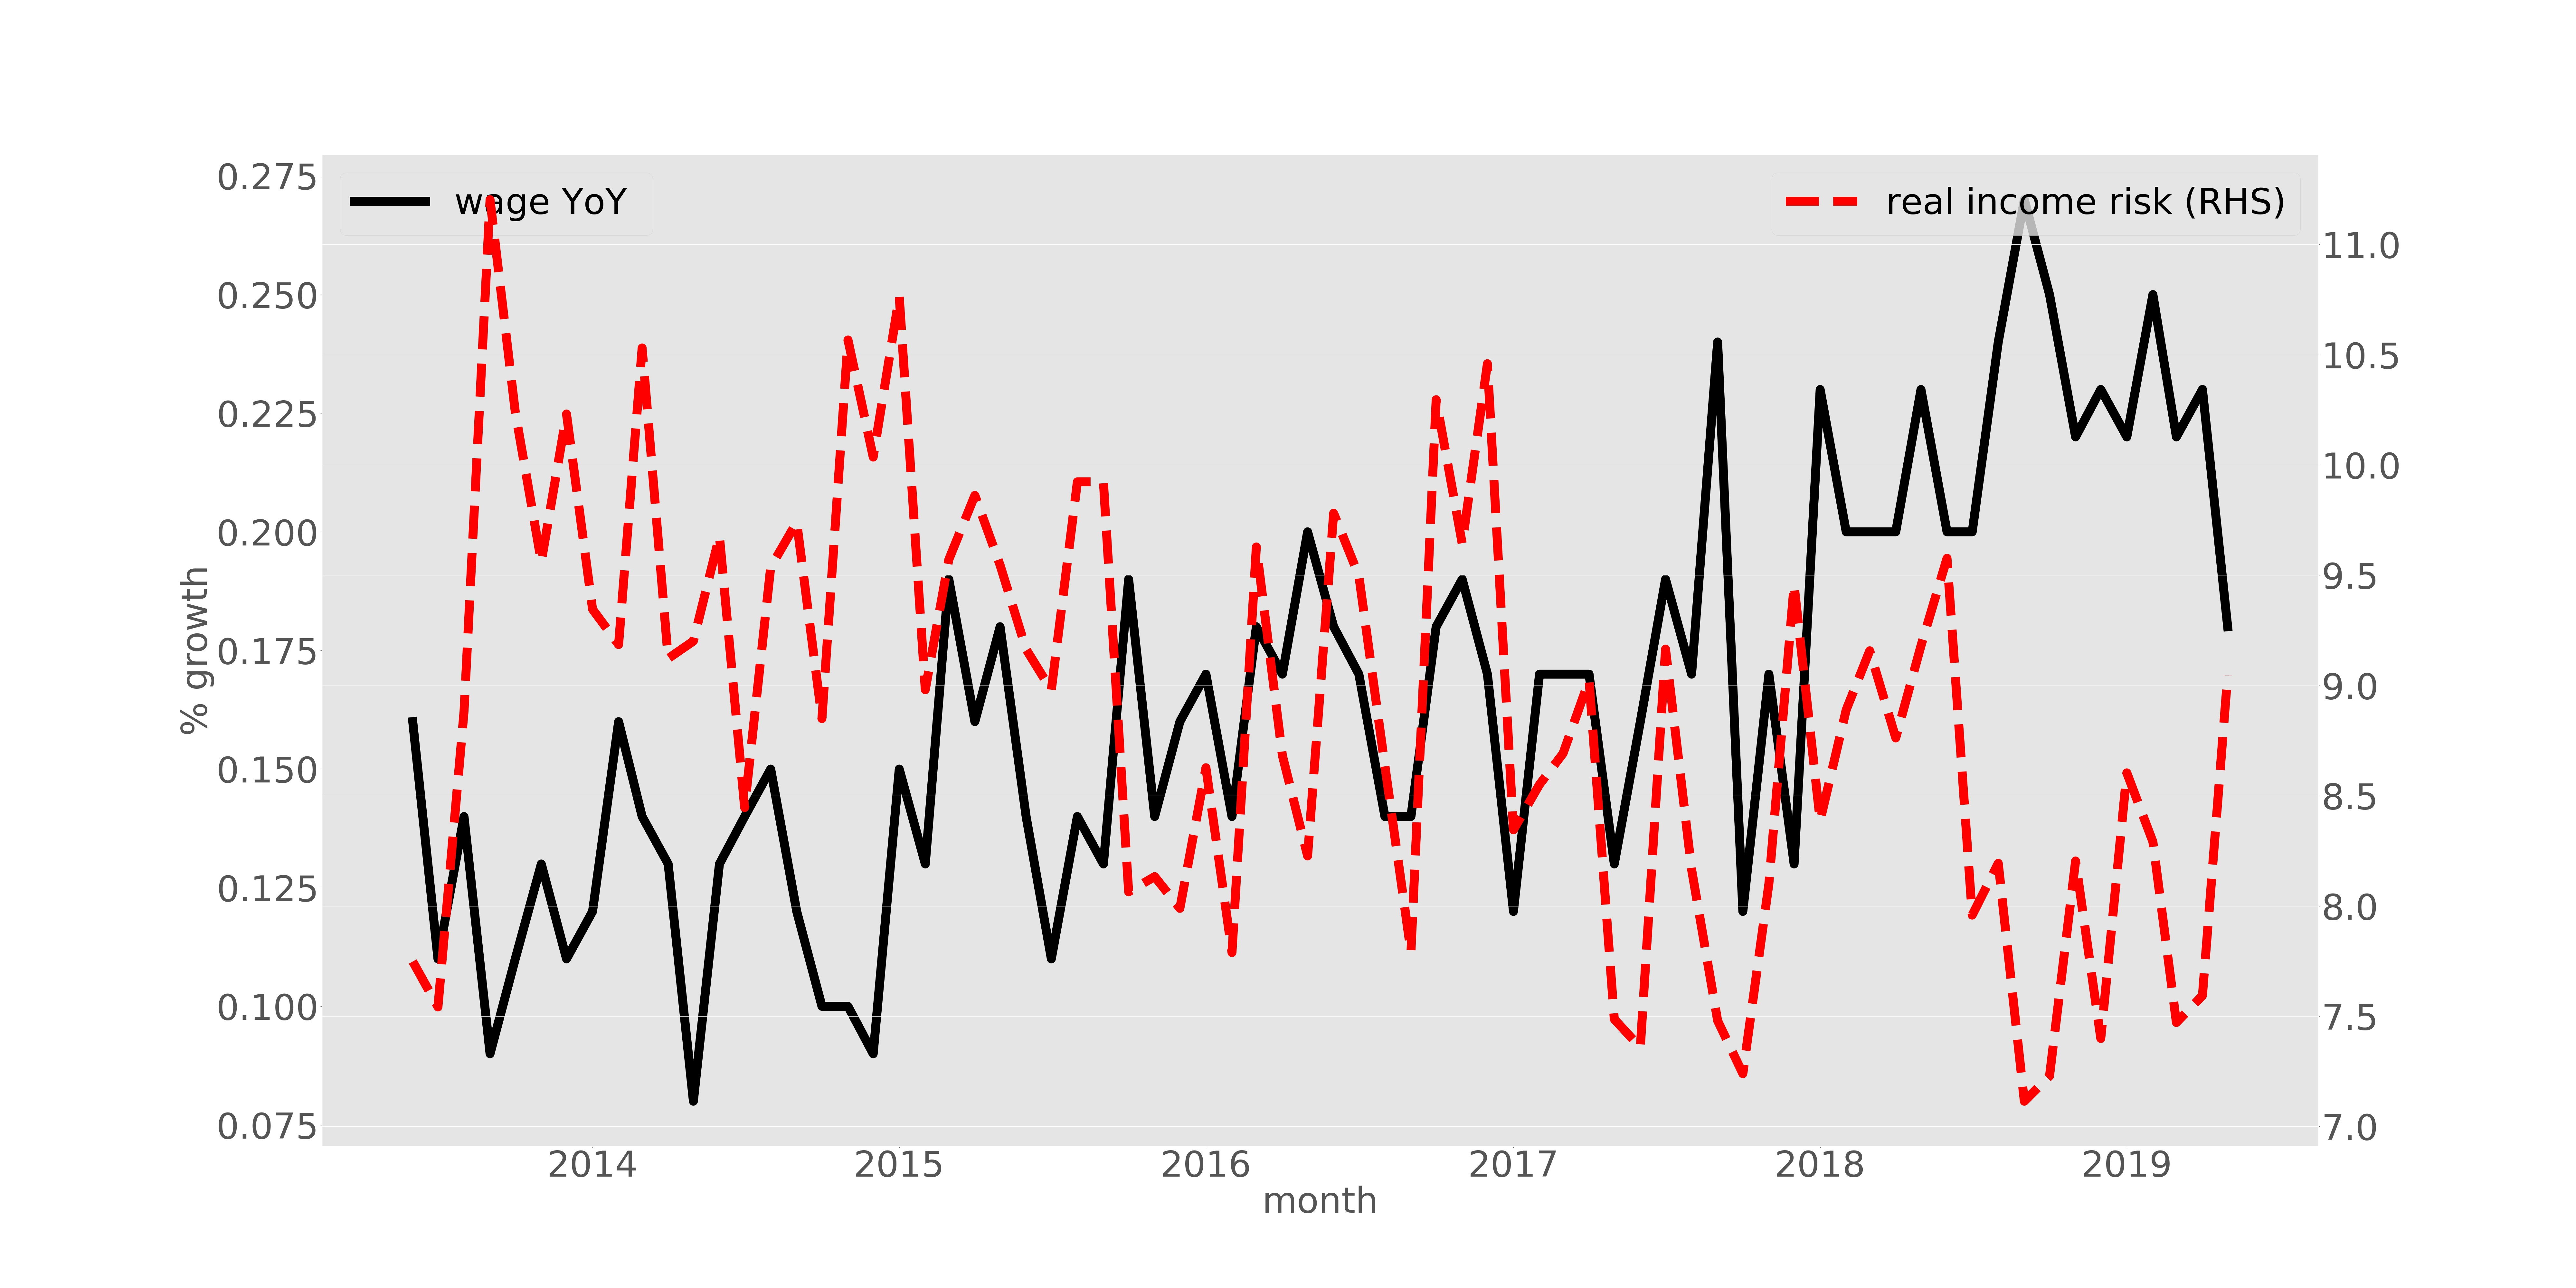
\includegraphics[width=\textwidth]{figures/tsMeanrvar_he.jpg}
%	\end{figure}
%\end{frame}



\begin{frame}{Perceived risks and current labor market condition}
	\begin{eqnarray*}
		\underbrace{\overline{\text{risk}_{t}}}_{\text{average perceived risk}} = \alpha + \textcolor{red}{\beta} \underbrace{(log(\text{wage}_{t-k}) - log(\text{wage}_{t-k-3}))}  _{\text{wage growth}}  + \epsilon_{i,t}	 \\
		\quad \forall k =1...6
	\end{eqnarray*}
	
	\begin{table}
		\centering
		%\caption{Correlation between Perceived Income Risks and Stock Market Return}
		\label{macro_corr_he}
		\adjustbox{max height=0.5\textheight, max width=\textwidth}{ 
			\begin{tabular}{lllllll}
				\hline
				k & varMean   & iqrMean   & rvarMean   & varMed   & iqrMed   & rvarMed   \\
				\hline
				1               & -2.046**  & -0.801*** & -10.437*** & -0.269   & -0.191   & -5.121*** \\
				2               & -3.823*** & -1.193*** & -12.287*** & -0.021   & 0.009    & -5.292*** \\
				3               & -2.942*** & -0.938*** & -9.642***  & -0.147   & -0.077   & -4.445*** \\
				4               & -3.261*** & -0.994*** & -9.021***  & -0.142   & -0.094   & -4.467*** \\
				5               & -2.312**  & -0.892*** & -6.792**   & -0.441** & -0.252*  & -4.718*** \\
				6               & -3.419*** & -1.207*** & -10.791*** & -0.412** & -0.274** & -5.466*** \\
				\hline
			\end{tabular}
		}
	\end{table}
	\end{frame}
	
	
	
	\begin{frame}{Perceived risks and current labor market condition}
	\begin{eqnarray*}
		\underbrace{\overline{\text{risk}_{s,t}} }_{\text{median perceived risk in state $s$}}= r + \textcolor{red}{\psi} \underbrace{LM_{s,t}}_{\text{state labor market condition}}  + \eta_{s,t}
	\end{eqnarray*}
		\begin{table}
			\centering
			%\caption{Correlation between Perceived Income Risks and Stock Market Return}
			\label{macro_corr_he_state}
			\adjustbox{max height=0.5\textheight, max width=\textwidth}{ 
			\begin{tabular}{lllll}
					\hline 
				& (1)                & (2)                & (3)               & (4)               \\
					\hline 
				& log(var) & log(risk) & log(iqr) & log(iqr) \\
				\hline 
			     wage growth & -0.05***           &                    & -0.03***          &                   \\
			     
				& (0.01)             &                    & (0.01)            &                   \\
				unemp rate &                    & 0.04*              &                   & 0.04***           \\
				&                    & (0.02)             &                   & (0.01)            \\
\hline 
				Observations      & 3529               & 3529               & 3546              & 3546              \\
				R-squared         & 0.023              & 0.020              & 0.025             & 0.028            \\
				\hline 
			\end{tabular}
		}
		\end{table}
	\end{frame}
	


\section{Conclusion}

\begin{frame}{Conclusion}
	\begin{itemize}
		\item Experience + Learning + \textcolor{blue}{Attribution} $\rightarrow$ Perception (Expectation) 
		\item Attribution is important because of
		\begin{itemize}
			\item imperfect understanding in both the size and the \textcolor{red}{nature} 
			\item forming perceptions about \textcolor{red}{second moments}, i.e. income risks
			\item certain attribution errors $\rightarrow$ \textcolor{red}{aggregate patterns}, i.e. counter-cyclical subjective risk 
		\end{itemize} 
	\end{itemize}
\end{frame}

\bibliographystyle{apalike}
\bibliography{PerceivedIncomeRisk}


\end{document}
